\chapter{Analyse et spécification des besoins}
\label{sec:unchapitre}

\begin{fquote}Dans ce chapitre, j’aborde les phases d’analyse et de spécification des besoins du projet, dans le but d’avoir une vision globale claire du comportement du projet ainsi que les attentes des utilisateurs.
 \end{fquote}

\clearpage

\section{Spécifications des besoins}

La spécification des besoins va nous permettre d’avoir une meilleure approche des utilisateurs, des fonctionnalités et de la relation entre les deux. Elle sera sous forme de besoins. Pour cela nous allons procéder comme ceci :
\begin{itemize}
	\item Identification des acteurs du nouveau système.
	\item Identification des besoins fonctionnels.
	\item Identification des besoins non fonctionnels .
\end{itemize}




\subsection{Identification des acteurs}
Un acteur est une personne, un matériel ou un logiciel qui interagit avec le système. L’analyse du présent projet commence par une identification des acteurs agissants sur les différentes parties du système. Les acteurs présentés dans la figure \ref{fig:profiles} sont des employés du clients en plus du serveur  qui est la solution adoptée par le client pour la communication et le partage des informations entre ces systèmes et départements .

\begin{figure}[ht]
  \centering
  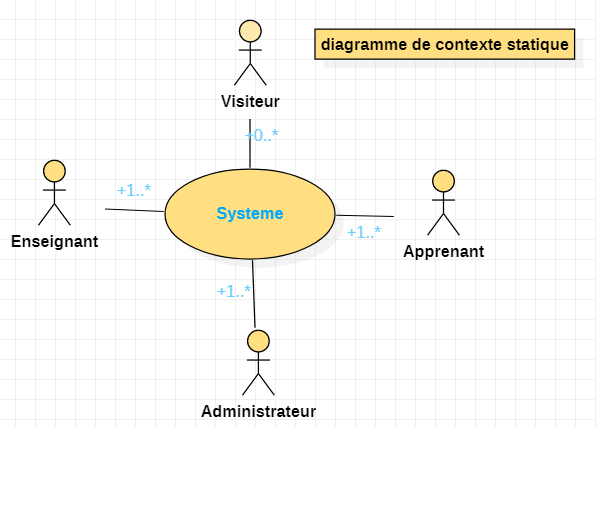
\includegraphics[width=14cm,height=8.5cm]{profiles}
  \caption{Héirarchie des profiles humaines.}
  \label{fig:profiles}
\end{figure}
\FloatBarrier
Le tableau \ref{actors} récapitule les acteurs en interaction avec le système en spécifiant le rôle de chacun avant de définir plus précisément leurs interactions avec le système en utilisant des diagrammes de cas d'utilisation.\\

\begin{table}[H]
\centering
\def\arraystretch{1.45}
\begin{tabular}{|c|c|}
\hline
\rowcolor{Gray} 
Acteur           & Fonction                                                                                                                                                                                                                                             \\ \hline
\rowcolor{LightCyan} 
Administrateur    & \begin{tabular}[c]{@{}c@{}} L’administrateur est la personne responsable de gérer la totalité du système.\\  \end{tabular} \\ \hline
\rowcolor{LightCyan} 



Enseignant & \begin{tabular}[c]{@{}c@{}} C’est un acteur principale qui interagit avec notre application.\\
C’est l’acteur qui a pour rôle de gérer les cours,\\ les travaux dirigés (TD) et les examens des
étudiants.\end{tabular}                   \\ \hline
\rowcolor{LightCyan} 



 
Apprenant & \begin{tabular}[c]{@{}c@{}}L’apprenant inscrit, il va pouvoir consulter \\les cours et faire les tests qui lui sont
	proposés.\\ L'apprenant peut avoir la possibilité de participer aux forums,\\ d'envoyer un
	message à un tuteur, \\à un autre apprenant ou même à l'administrateur.\\ Ainsi la possibilité
	de discussion en ligne avec le tuteur,\\ la modification de son profil et la consultation de
	sesrésultats.\end{tabular}                   \\ \hline
\rowcolor{LightCyan} 



Visiteur & \begin{tabular}[c]{@{}c@{}}N’importe quel visiteur qui \\veut télécharger des cours via un compte personnelle a
	condition \\ de faire les inscriptions pour avoir un compte.\end{tabular}                   \\ \hline
\rowcolor{LightCyan} 
\end{tabular}
\caption{Acteurs en interaction avec le système}
\label{actors}
\end{table}
\clearpage
\subsection{Les besoins fonctionnels}
Les besoins fonctionnels expriment une action que doit effectuer le système en réponse à une demande .\\
Les besoins principaux à couvrir par le système sont les suivants :\\
{\color{cyan} Si l’acteur est un Administrateur, il peut :
}

\begin{itemize}
	\item \underline{S’authentifier}  :l’Administarateur entre son « username » et son « password » avant d’accéder à l’application pour assurer la confidentialité des informations.
	\item \underline{Gérer les comptes des utilisateurs} : l’Administrateur peut ajouter des comptes pour les
	nouveaux Utilisateurs(Enseignant ou Etudiant) , modifier leurs informations et supprimer
	les comptes des anciens utilisateurs.
\end{itemize}
{\color{cyan}Si l’acteur est un Enseignant, il peut :}
\begin{itemize}
	\item \underline{Gérer les Matières} :l’Enseignant peut ajouter, modifier et supprimer les matières.
	\item  \underline{Gérer les Cours }:l’Enseignant peut ajouter, modifier et supprimer les cours.

	\item \underline{Gérer les Traveaux dirigés(TD) }:l’Enseignant peut ajouter,modifier et supprimer les Traveaux dirigés(TD).
	\item \underline{Gérer les Examens }:l’Enseignant peut ajouter des examens en choisissant une durée de
	temps determiné.
\end{itemize}
{\color{cyan}Si l’acteur est un Etudiant, il peut :}
\begin{itemize}
	\item \underline{Consulter les Cours} :l’Etudiant peut consulter et télecharger les cours.
	\item \underline{Consulter les Traveaux dirigés(TD) }:l’Etudiant peut consulter et télecharger les Traveaux
	dirigés(TD).
	\item \underline{Passer les Examens }:l’Etudiant peut passer les examens en respectant une durée de temps
	determinée.
\end{itemize}

\subsection{Les besoins non fonctionnels}
Les besoins non fonctionnels impressionne directement sur déroulement réelle de l’application. Ce sont des besoins techniques décrivant la majorité des contraintes (qu’on a déjà
approuvée dans le chapitre précèdent) auxquelles est soumis le système pour sa réalisation et
son bon fonctionnement. Pour cela l’ensemble des extensions à réaliser doivent respecter les besoins suivants :
%Les besoins non fonctionnels représentent les exigences implicites auquel le système doit répondre. Parmi ces besoins on cite :

\begin{itemize}
	\item \underline{La Sécurité} : La solution proposée permet à l’utilisateur une navigation sécurisée.
	Elle n’est accessible qu’avec une authentification.
	\item \underline{Ergonomie de l’interface }: L’ergonomie est un élément important de l’application : les
	écrans de saisie doivent être clairs, organisés avec cohérence, de façon à ce qu’une prise
	en main soit la plus rapide possible.
	\item \underline{
Maintenance }: L’une des plus importantes besoins de notre application est la facilité de
	modification pour s’adopter aux nouveaux besoins.
	\item \underline{Portabilité} : L’application doit être accessible via n’importe quel navigateur.

\end{itemize}

%\section{Analyse des besoins fonctionnels}
%L’analyse des besoins est une étape très importante dans le processus de l’étude et le développement des systèmes d’informations. Cette partie identifie l’ensemble des acteurs qui interagissent avec le système et définit l’ensemble des cas d’utilisation de ce dernier en se basant sur les diagrammes UML.
\section{Backlog produit}
Le Backlog produit est une liste ordonnée de tout ce qui pourrait être nécessaire dans un produit et constitue l’unique source d'exigences pour toutes les modifications apportées au produit. Le Product Owner est responsable du Backlog produit, y compris son contenu, sa disponibilité et son ordonnancement.\\
 Ses toutes premières moutures ne font qu’esquisser les besoins tels qu’initialement connus et compris. Le Backlog Produit évolue au fur et à mesure que le produit et le contexte dans lequel il sera utilisé évoluent. Le Backlog Produit est dynamique; il change constamment pour identifier ce que le produit requiert pour être approprié, compétitif et utile. Tant et aussi longtemps qu’un produit existe, son Backlog Produit correspondant existe.\\
 Les caractéristiques fonctionnelles sont appelées
 des histoires utilisateurs (user story). Les user stories sont caractérisés par :\\
\begin{itemize}[label=$\square$,leftmargin=* ,parsep=0cm,itemsep=0cm,topsep=0cm]
    \item \textit{\textbf{Identifiant}} Il détermine un identifiant unique pour l’histoire en question.\\
 	
 	\item \textit{\textbf{Description}}Elle décrit le besoin d’un acteur.\\
 	
 	\item \textit{\textbf{Critères d’acceptation}}À chaque user story sont associés des critères permettant au client
 	de tester l’histoire. Ces critères d’acceptation peuvent être formalisés, pour aller un peu plus
 	loin dans l’aide fournie à l’équipe que l’énoncé de ces critères.\\
 
 	\item \textit{\textbf{Estimation}}Est une estimation de la complexité, elle est une valeur entière qui appartient à la suite de Fibonacci.
 	 
 	
 	\item \textit{\textbf{Priorité}}  Les priorités sont utilisées pour définir l’ordre de réalisation, elles permettent de
 	constituer le flux de stories qui va alimenter l’équipe. Pour prioriser nos user stories, nous
 	avons pris en compte les critères suivant :
 	\begin{enumerate}
 		\item \textit{La valeur apportée (Business Value)}
 		\item \textit{La fréquence d’utilisation}
 		\item \textit{La réduction des risques}
 		\item \textit{L’incertitude sur des besoins des utilisateurs qu’un user story permettra de diminuer}
 		\item \textit{La contribution à la qualité. Les travaux visant à garantir la qualité du produit devraient être prioritaires}
 		\item \textit{Les dépendances entre stories}
 	\end{enumerate}
 	
Lors de la création de notre Backlog, nous avons essayé de produire des user stories qui respectent
les critères réunies dans le mot INVEST, c’est à dire
	\begin{itemize}	
\item[$\star$] Independant : Ne dépend de rien (réduire les liens entre items)
\item[$\star$] Negociable : Je n’ai pas une solution technique figée
\item[$\star$] Valuable : pour le client (a une valeur Business)
\item[$\star$] Estimable : Estimation en complexité
\item[$\star$] Small / Sized Appropriately : De petite taille (A définir en interne de l’entreprise)
\item[$\star$] Testable : Pour la validation de l’item
\end{itemize}
\end{itemize}
 \bigskip
 

\subsection{Planification des Sprints}
-Duree des Sprints
\subsection{Backlog des Sprints}
Le Sprint Backlog comporte la liste des tâches du Sprint (son périmètre donc) ainsi que la charge de travail associée à ces dernières. Chaque jour, le Reste A Faire de chaque tâche est actualisé par l’équipe de développement afin de tracer le graphique d’avancement de Sprint.


\section{Diagrammes des cas d'utilisation global}
Le modèle des cas d’utilisation décrit les fonctionnalités d’un système d’un point de vue utilisateur, sous la forme d’actions et de réactions ; l’ensemble des fonctionnalités est déterminé en examinant les besoins fonctionnels de tous les utilisateurs potentiels.\\
Ainsi, pour construire notre modèle, nous allons organiser les cas d’utilisation et les regrouper en ensembles fonctionnels cohérents. Pour ce faire, nous utilisons le concept général d’UML, le package.

\subsubsection{Le profil Admin :}
Ce diagramme illustre le cas d’utilisation générale de notre système. Ces cas d’utilisation seront par la suite expliqués en détaille. (voir la figure \ref{fig:UseCaseAdmin}):
\begin{figure}[ht]
  \centering
  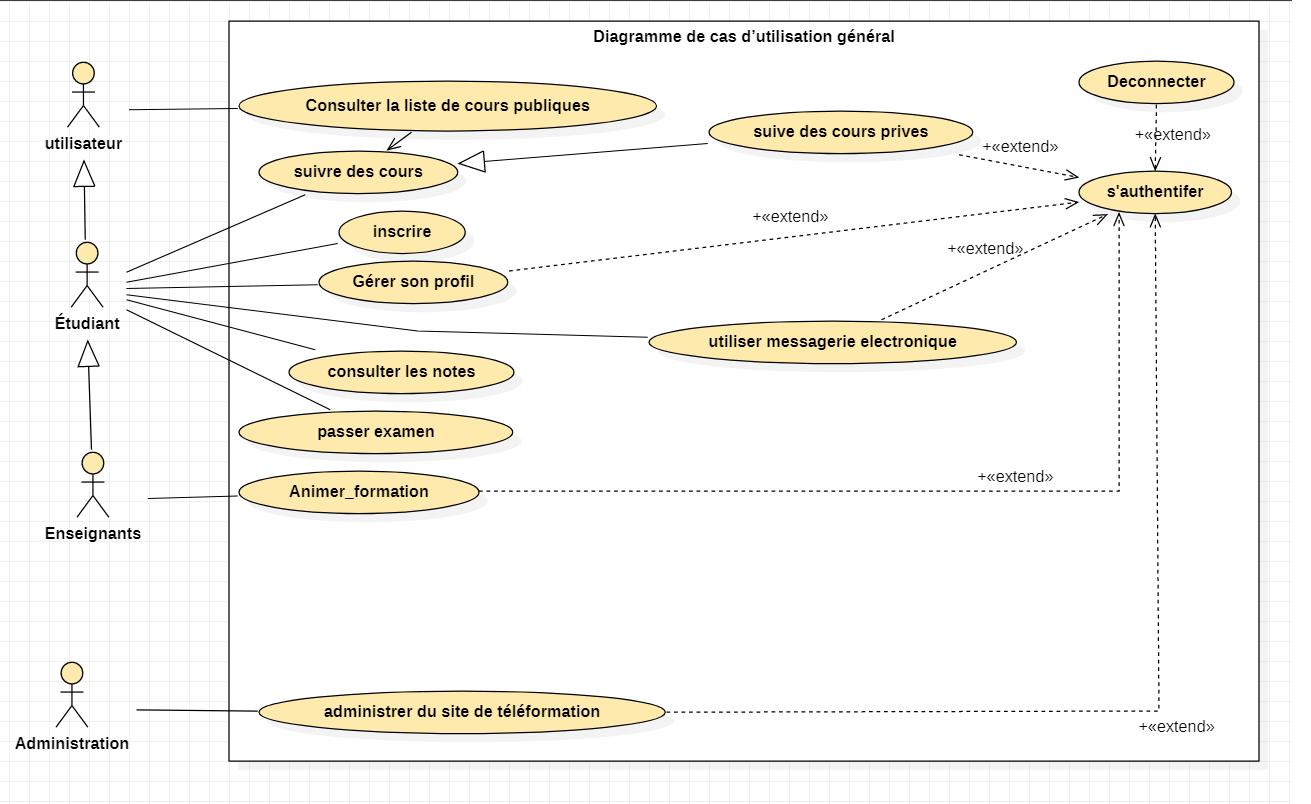
\includegraphics[width=18cm,height=12cm]{UseCaseAdmin.png}
  \caption{Les cas d'utilisation global.}
  \label{fig:UseCaseAdmin}
\end{figure}
\FloatBarrier
\begin{itemize}

\item[$\bullet$] \textbf{Cas d’utilisation S’authentifier :} permet aux utilisateurs de se connecter au système avec leurs logins et mots de passe afin de sécuriser la platforme.
\medskip
    \begin{itemize}
    \item \textit{\textbf{Objectif :}}  Cette fonctionnalité permet aux différents acteurs de se connecter. 

    \item \textit{\textbf{Acteur :}} Tous les acteurs

    \item \textit{\textbf{Pré-condition  :}} L’utilisateur existe dans la base de données.
\item \textit{\textbf{Post-conditions   :}} Utilisateur authentifié.
    \item \textit{\textbf{Scénario nominal :}}
         \begin{enumerate}
             \item L’acteur saisit son login et son mot de passe. 
             \item Le système vérifie les informations saisies. 
             \item Le système trouve que les informations saisies sont valides.  
             \item Le système vérifie le rôle de l’acteur.  
             \item Le système connecte l’acteur à son espace.
         \end{enumerate}
    \item \textit{\textbf{Scénario d'erreur :}} 
         \begin{enumerate}
             \item L’acteur saisit son login et son mot de passe. 
             \item Le système vérifie les informations saisies.   
             \item Le système trouve que les informations saisies sont invalides.  
             \item Le système demande à l’acteur de vérifier les informations saisies.
         \end{enumerate}
    \end{itemize}

\bigskip

\item[$\bullet$] \textbf{Cas d’utilisation Gérer les employés :} L’administrateur prend en charge la gestion des utilisateurs de la plat-forme :
\medskip
    \begin{itemize}
    \item \textit{\textbf{Objectif :}}  Cette fonctionnalité permet à l’administrateur de gérer les utilisateurs du PIM qui sont des employés du client.

    \item \textit{\textbf{Acteur :}} Administrateur

    \item \textit{\textbf{Pré-condition  :}} L’acteur se connecte au système. 

    \item \textit{\textbf{Scénarios nominaux :}}
         \begin{enumerate}
             \item \textit{Ajouter un utilisateur.}
                    \begin{itemize}
                       \item[$\star$]  L’acteur saisit les informations de l’utilisateur. 
                       \item[$\star$] Le système confirme à l’administrateur l’enregistrement de l’utilisateur.
                       \item[$\star$] Le système affiche la liste des utilisateurs contenant l’utilisateur ajouté.
                    \end{itemize}
             \item \textit{Modifier un utilisateur.}
                    \begin{itemize}
                       \item[$\star$] L’acteur affiche la liste des utilisateurs. 
                       \item[$\star$] L’acteur sélectionne l’utilisateur à modifier. 
                       \item[$\star$] Le système affiche les informations de l’utilisateur sélectionné
                       \item[$\star$] L’acteur modifie les champs concernés. 
                       \item[$\star$] L’acteur valide ses modifications. 
                       \item[$\star$] Le système confirme à l’acteur la mise à jour des informations.
                       \item[$\star$] Le système affiche la liste des utilisateurs contenant l’utilisateur modifié.
                    \end{itemize}
             \item \textit{Supprimer un utilisateur :}
                    \begin{itemize}
                       \item[$\star$] L’acteur affiche la liste des utilisateurs. 
                       \item[$\star$] L’acteur sélectionne l’utilisateur à supprimer. 
                       \item[$\star$] Le système alerte l’acteur sur son action. 
                       \item[$\star$] L’acteur valide son action.
                       \item[$\star$] Le système confirme à l’acteur la suppression de l’utilisateur.
                    \end{itemize}
                \item \textit{Chercher des utilisateurs :}
                    \begin{itemize}
                       \item[$\star$] L’acteur affiche la liste des utilisateurs. 
                       \item[$\star$] L’acteur clique sur le volet de recherche.
                       \item[$\star$] L'acteur choisit les critères de recherche. 
                       \item[$\star$] L’acteur lance la recherche.
                       \item[$\star$] Le système affiche les résultats de recherche.
                    \end{itemize}
         \end{enumerate}
    \end{itemize}
    \bigskip

\item[$\bullet$] \textbf{Cas d’utilisation Gérer les catégories :} L’administrateur peut gérer les catégories qui sert a classifier les produits selon leurs critères et typologies :
\medskip
    \begin{itemize}
    \item \textit{\textbf{Objectif :}}  Cette fonctionnalité permet à l’administrateur de gérer les catégories des produits disponibles dans le PIM.

    \item \textit{\textbf{Acteur :}} Administrateur

    \item \textit{\textbf{Pré-condition  :}} L’acteur se connecte au système. 

    \item \textit{\textbf{Scénarios nominaux :}}
         \begin{enumerate}
             \item \textit{Ajouter une catégorie.}
                    \begin{itemize}
                       \item[$\star$]  L’acteur saisit les informations de la catégorie. 
                       \item[$\star$] Le système confirme à l’administrateur l’enregistrement de la catégorie.
                       \item[$\star$] Le système affiche la liste des catégories contenant la catégorie ajoutée.
                    \end{itemize}
             \item \textit{Modifier une catégorie.}
                    \begin{itemize}
                       \item[$\star$] L’acteur affiche la liste des catégories. 
                       \item[$\star$] L’acteur sélectionne la catégorie à modifier. 
                       \item[$\star$] Le système affiche les informations de la catégorie sélectionnée
                       \item[$\star$] L’acteur modifie les champs concernés. 
                       \item[$\star$] L’acteur valide ses modifications. 
                       \item[$\star$] Le système confirme à l’acteur la mise à jour des informations.
                    \end{itemize}
             \item \textit{Supprimer une catégorie :}
                    \begin{itemize}
                       \item[$\star$] L’acteur affiche la liste des catégories. 
                       \item[$\star$] L’acteur sélectionne la catégorie à supprimer. 
                       \item[$\star$] Le système alerte l’acteur sur son action. 
                       \item[$\star$] L’acteur valide son action.
                       \item[$\star$] Le système confirme à l’acteur la suppression de la catégorie.
                    \end{itemize}
                \item \textit{Affecter/désaffecter des produits à une catégorie :}
                    \begin{itemize}
                        \item[$\star$] L’acteur affiche la liste des catégories. 
                       \item[$\star$] L’acteur sélectionne la catégorie souhaitée. 
                       \item[$\star$] Le système affiche les informations de la catégorie sélectionnée
                       \item[$\star$] L’acteur ouvre l'onglet des produits inclut dans la catégorie. 
                       \item[$\star$] L’acteur ajoute/supprime des produits à/de la catégorie.
                       \item[$\star$] L’acteur valide ses modifications.
                       \item[$\star$] Le système confirme à l’acteur la mise à jour des informations.
                    \end{itemize}
                \item \textit{Chercher une catégorie :}
                    \begin{itemize}
                       \item[$\star$] L’acteur affiche la liste des catégories. 
                       \item[$\star$] L’acteur sélectionne ouvre le voler de recherche. 
                       \item[$\star$] L'utilisateur choisit les critères de recherche. 
                       \item[$\star$] L’acteur lance la recherche.
                       \item[$\star$] Le système affiche la liste des catégories conformes à la recherche.
                    \end{itemize}
         \end{enumerate}
    \end{itemize}
    \bigskip

    


    \end{itemize}
        \bigskip

       
                   
\section{Diagrammes de classes global}
Le diagramme de classes est un schéma utilisé en génie logiciel pour présenter les classes et les interfaces des systèmes ainsi que les différentes relations entre celles ci. Ce diagramme fait
partie de la partie statique d’UML car il fait abstraction des aspects temporels et dynamiques.
Une classe est un ensemble de fonctions et de données (attributs) qui sont liées ensembles par un champ sémantique [N4]. Dans ce qui suit nous allons décrire le diagramme de classes relatif à notre application.
 \ref{fig:UseCaseCatalogManager}).
\begin{figure}[ht]
  \centering
  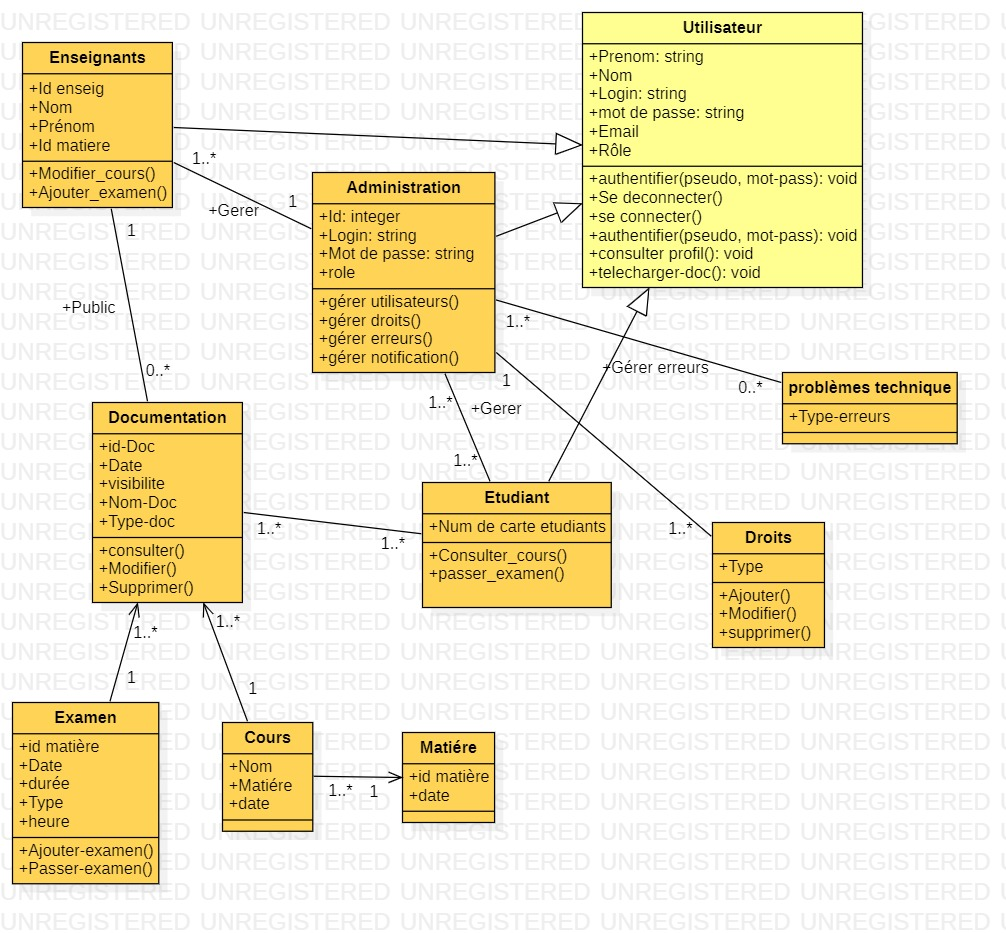
\includegraphics[width=18cm,height=8cm]{UseCaseCatalogManager.jpg}
  \caption{Diagrammes de classes global.}
  \label{fig:UseCaseCatalogManager}
\end{figure}
\FloatBarrier






              
\subsection{Conclusion}
Le but de ce chapitre était de définir et d’analyser l’ensemble des besoins fonctionnels  de notre solution. Cette étape est primordiale dans le développement d’un projet informatique puisque elle nous permet de définir le périmètre fonctionnel du projet, et de garantir la couverture de l’ensemble des fonctionnalités recensées.
